% ============================================================================
% Resultados do benchmark CGV-Web na máquina de referência (RTX 4070 Ti)
% current (nova) x baseline (antiga). MESCLA por réplica de todas as execuções
% completas em bench/dados/rtx4070ti/ (3 current + 2 baseline de 78 s, mais 1
% varredura rápida de conferência). Gerado a partir de
% bench/resultados/rtx4070ti/stats.json (recomputado dos frames brutos).
% Figuras: mesma pasta deste arquivo. Compilável isoladamente
% (pdflatex/tectonic resultados.tex, de dentro desta pasta).
% ============================================================================
\documentclass[11pt,a4paper]{article}
\usepackage[utf8]{inputenc}
\usepackage[T1]{fontenc}
\usepackage[brazil]{babel}
\usepackage{graphicx}
\usepackage{booktabs}
\usepackage[margin=2.5cm]{geometry}
\graphicspath{{./}}

\title{CGV-Web: impacto das otimiza\c{c}\~oes de renderiza\c{c}\~ao\\ \large Resultados do benchmark automatizado (RTX~4070~Ti, dados mesclados)}
\author{}
\date{}

\begin{document}
\maketitle

\section{Metodologia}

O desempenho foi medido por um \emph{runner} externo ao aplicativo, que executa um la\c{c}o
\texttt{request\-Animation\-Frame} pr\'oprio e registra o timestamp bruto de cada quadro
apresentado; o m\'etodo \'e id\^entico nas duas vers\~oes e n\~ao instrumenta o c\'odigo medido.
Ambas as vers\~oes rodaram na mesma m\'aquina (NVIDIA RTX~4070~Ti, Chrome com limite de FPS
destravado, \emph{viewport} $1920\times1080$, \emph{devicePixelRatio}~1), sobre os mesmos sete
eventos reais do ATLAS (23{,}3~mil a 57{,}4~mil c\'elulas de calor\'imetro), em tr\^es
cen\'arios: \emph{tour} (volta autom\'atica padronizada da c\^amera, $3\times78$~s por evento),
\emph{corte parado} e \emph{arraste do corte} (8~s por eixo).

\paragraph{Mescla das execu\c{c}\~oes (agrega\c{c}\~ao por r\'eplica).}
Trata-se cada su\'ite completa como uma r\'eplica: por cen\'ario e vers\~ao calcula-se a
estat\'istica de cada execu\c{c}\~ao (agrupando suas repeti\c{c}\~oes) e agrega-se pela
\emph{m\'edia entre execu\c{c}\~oes}, com peso igual, o que evita favorecer execu\c{c}\~oes mais
r\'apidas (que geram mais quadros) e exp\~oe a variabilidade entre sess\~oes. Nesta m\'aquina
entram no pool \textbf{tr\^es} execu\c{c}\~oes completas do \emph{current} e \textbf{duas} do
\emph{baseline} (ciclo de 78~s); uma varredura r\'apida adicional do \emph{baseline} (ciclo de
10~s) serve apenas de confer\^encia de reprodutibilidade. As c\'elulas efetivamente
renderizadas conferem entre as vers\~oes (diferen\c{c}a de 128 c\'elulas, at\'e $0{,}65\%$, a
favor da vers\~ao antiga) e os tri\^angulos por quadro diferem cerca de $7\%$, tamb\'em a favor
da antiga --- ambas conservadoras.

\section{Resultados}

\begin{table}[htbp]
\centering
\caption{FPS mediano (m\'edia entre execu\c{c}\~oes), faixa do \emph{current} entre
execu\c{c}\~oes, \emph{speedup} e \emph{draw calls} por quadro. ``b'' = baseline (antiga),
``c'' = current (nova).}
\label{tab:rtx}
\small
\begin{tabular}{llrrcrr}
\toprule
Cen\'ario & Evento & C\'elulas & FPS b$\to$c & Nova (faixa) & Speedup & Draws b$\to$c \\
\midrule
tour & 517743$\cdot$363 & 23\,349 & 47{,}6 $\to$ 370 & 294--417 & 7{,}8$\times$ & 13\,835 $\to$ 46 \\
tour & 518084$\cdot$443 & 23\,612 & 47{,}6 $\to$ 355 & 294--400 & 7{,}5$\times$ & 13\,974 $\to$ 58 \\
tour & 518084$\cdot$891 & 25\,825 & 47{,}5 $\to$ 355 & 294--400 & 7{,}5$\times$ & 14\,064 $\to$ 66 \\
tour & 516761$\cdot$342 & 39\,043 & 46{,}3 $\to$ 318 & 263--357 & 6{,}9$\times$ & 14\,587 $\to$ 160 \\
tour & 520526$\cdot$948 & 40\,976 & 44{,}3 $\to$ 304 & 256--333 & 6{,}9$\times$ & 15\,243 $\to$ 195 \\
tour & 520249$\cdot$978 & 43\,367 & 44{,}7 $\to$ 316 & 256--357 & 7{,}1$\times$ & 15\,198 $\to$ 192 \\
tour & 520534$\cdot$398 & 57\,359 & 40{,}8 $\to$ 306 & 270--345 & 7{,}5$\times$ & 16\,860 $\to$ 185 \\
corte parado & 520534$\cdot$398 & 57\,359 & 41{,}5 $\to$ 289 & 250--313 & 7{,}0$\times$ & 16\,864 $\to$ 189 \\
arraste $\theta$ & 520534$\cdot$398 & 57\,359 & 8{,}3 $\to$ 242 & 213--263 & 29{,}0$\times$ & 17\,112 $\to$ 200 \\
arraste $z$ & 520534$\cdot$398 & 57\,359 & 8{,}5 $\to$ 242 & 213--256 & 28{,}5$\times$ & 17\,370 $\to$ 192 \\
arraste raio & 520534$\cdot$398 & 57\,359 & 10{,}0 $\to$ 242 & 213--256 & 24{,}1$\times$ & 17\,339 $\to$ 199 \\
\midrule
\multicolumn{5}{l}{M\'edia geom\'etrica dos \emph{speedups} (11 cen\'arios)} & 10{,}4$\times$ & \\
\bottomrule
\end{tabular}
\end{table}

\paragraph{Vis\~ao geral.}
Agregando as cinco execu\c{c}\~oes completas, a vers\~ao nova \'e mais r\'apida em todos os 11
cen\'arios comuns, com ganho t\'ipico (m\'edia geom\'etrica) de \textbf{10{,}4$\times$} no FPS
mediano (Tabela~\ref{tab:rtx}, Figura~\ref{fig:speedup-rtx}). O ganho tem dois regimes. Na
visualiza\c{c}\~ao passiva, o \emph{tour} e o corte parado ficam entre 6{,}9$\times$ e
7{,}8$\times$ (m\'edia geom\'etrica de 7{,}3$\times$ nos \emph{tours} e 7{,}0$\times$ no corte
parado): a vers\~ao antiga n\~ao atinge 60~FPS em nenhum evento (40{,}8 a 47{,}6~FPS), enquanto
a nova opera entre 289 e 370~FPS de m\'edia, com 1\%~low de 236 a 291~FPS. No \emph{arraste do
corte}, o caso interativo cr\'itico, o ganho vai de 24{,}1$\times$ a 29{,}0$\times$ (m\'edia
geom\'etrica de 27{,}1$\times$): a antiga ca\'ia para 8 a 10~FPS medianos (1\%~low de 6~FPS;
\emph{frame-time} mediano de 98 a 120~ms), efetivamente inutiliz\'avel, enquanto a nova sustenta
242~FPS (Figura~\ref{fig:drag-rtx}).

\paragraph{Mecanismo.}
A causa dominante \'e a elimina\c{c}\~ao do gargalo de CPU por \emph{draw calls}
(Figura~\ref{fig:mecanismo-rtx}): a antiga emite de 13{,}8~mil a 17{,}4~mil ordens de desenho
por quadro, n\'umero que cresce com a quantidade de c\'elulas do evento; a nova agrupa as
c\'elulas em lotes e emite de 46 a 200 (redu\c{c}\~ao de duas ordens de grandeza), desenhando
praticamente a mesma geometria. Com a CPU fora do caminho cr\'itico, a vaz\~ao \'util da GPU
sobe de 20--108 para 565--881~Mtri/s, cerca de 10$\times$. No arraste soma-se a mudan\c{c}a de
algoritmo: o corte passou a ser aplicado na GPU, pela atualiza\c{c}\~ao de um par\^ametro, em
vez de recalculado na CPU a cada movimento do mouse.

\paragraph{Lat\^encia e regularidade.}
O ganho n\~ao \'e apenas de m\'edia; a cauda encolhe drasticamente. No \emph{tour} do evento
mais pesado, o p99 do \emph{frame-time} cai de 29{,}5~ms para cerca de 4~ms. Nos arrastes, o p99
da antiga fica em 160--173~ms; o da nova, entre 18 e 19~ms de m\'edia entre execu\c{c}\~oes
(algumas execu\c{c}\~oes mant\^em a cauda em ${\sim}7$~ms, outras a levam a ${\sim}40$~ms),
ainda muito abaixo da antiga. O eixo azimutal $\varphi$, in\'edito na vers\~ao nova e por isso
sem baseline de compara\c{c}\~ao, mant\'em 232~FPS medianos com cauda maior (1\%~low de 67~FPS;
p99 de 29~ms), associada a picos ao recruzar a emenda de $\varphi$ em $\pm\pi$. Fora do la\c{c}o
de renderiza\c{c}\~ao, abrir um evento (an\'alise do JiveXML) ficou tipicamente 5{,}4$\times$
mais r\'apido (o pior caso cai de 5{,}4~s para 0{,}6~s), ao custo da prepara\c{c}\~ao da
geometria ao iniciar o aplicativo, que subiu de ${\sim}0{,}4$~s para ${\sim}1{,}0$~s.

\paragraph{Reprodutibilidade entre execu\c{c}\~oes.}
As r\'eplicas revelam que a vers\~ao antiga \'e muito est\'avel entre execu\c{c}\~oes (as duas
medi\c{c}\~oes completas concordam dentro de ${\sim}4\%$, e a varredura r\'apida de 10~s
reproduz o mesmo patamar de ${\sim}45$~FPS), ao passo que a vers\~ao nova, por rodar a centenas
de FPS, \'e mais sens\'ivel a varia\c{c}\~oes da m\'aquina (carga de fundo, aquecimento): entre
as tr\^es execu\c{c}\~oes completas o FPS mediano dos \emph{tours} varia at\'e $42\%$ (256 a
417~FPS conforme o evento e a execu\c{c}\~ao), como mostra a Figura~\ref{fig:repro-rtx}. Por
isso os valores deste relat\'orio usam a m\'edia entre execu\c{c}\~oes, uma estimativa
conservadora: mesmo a execu\c{c}\~ao mais lenta da nova (256~FPS nos \emph{tours}, 213~FPS no
arraste) mant\'em o ganho em ${\sim}5$--$6\times$ na visualiza\c{c}\~ao e ${\sim}25\times$ no
arraste.

\paragraph{Amea\c{c}as \`a validade.}
(i)~A carga n\~ao \'e bit-id\^entica: a vers\~ao nova renderiza 128 c\'elulas a mais
($+0{,}24\%$ a $+0{,}65\%$) e cerca de $7\%$ mais tri\^angulos por quadro; ambas as
diferen\c{c}as pesam contra a vers\~ao nova. (ii)~No arraste, o \^angulo de abertura registrado
do corte difere (180$^\circ$ na antiga, 110{,}2$^\circ$ na nova); como c\'elulas renderizadas e
tri\^angulos por quadro conferem, o efeito \'e de segunda ordem frente ao ganho de 24$\times$ a
29$\times$. (iii)~O arraste tem uma repeti\c{c}\~ao de 8~s por eixo, contra tr\^es
repeti\c{c}\~oes de 78~s nos \emph{tours}, e sua cauda \'e a mais sens\'ivel entre
execu\c{c}\~oes. (iv)~GPU, navegador, resolu\c{c}\~ao e trajet\'oria de c\^amera id\^enticos,
verificados nos metadados de todas as execu\c{c}\~oes.

\begin{figure}[htbp]
  \centering
  
\includegraphics[width=\linewidth]{01_speedup.png}
  \caption{\emph{Speedup} do FPS mediano por cen\'ario (m\'edia entre execu\c{c}\~oes, escala
  log). Ganho t\'ipico de 10{,}4$\times$; arrastes de corte entre 24$\times$ e 29$\times$.}
  \label{fig:speedup-rtx}
\end{figure}

\begin{figure}[htbp]
  \centering
  
\includegraphics[width=\linewidth]{04_mecanismo.png}
  \caption{Mecanismo do ganho: duas ordens de grandeza menos \emph{draw calls} por quadro nos
  \emph{tours}, para a mesma carga de c\'elulas.}
  \label{fig:mecanismo-rtx}
\end{figure}

\begin{figure}[htbp]
  \centering
  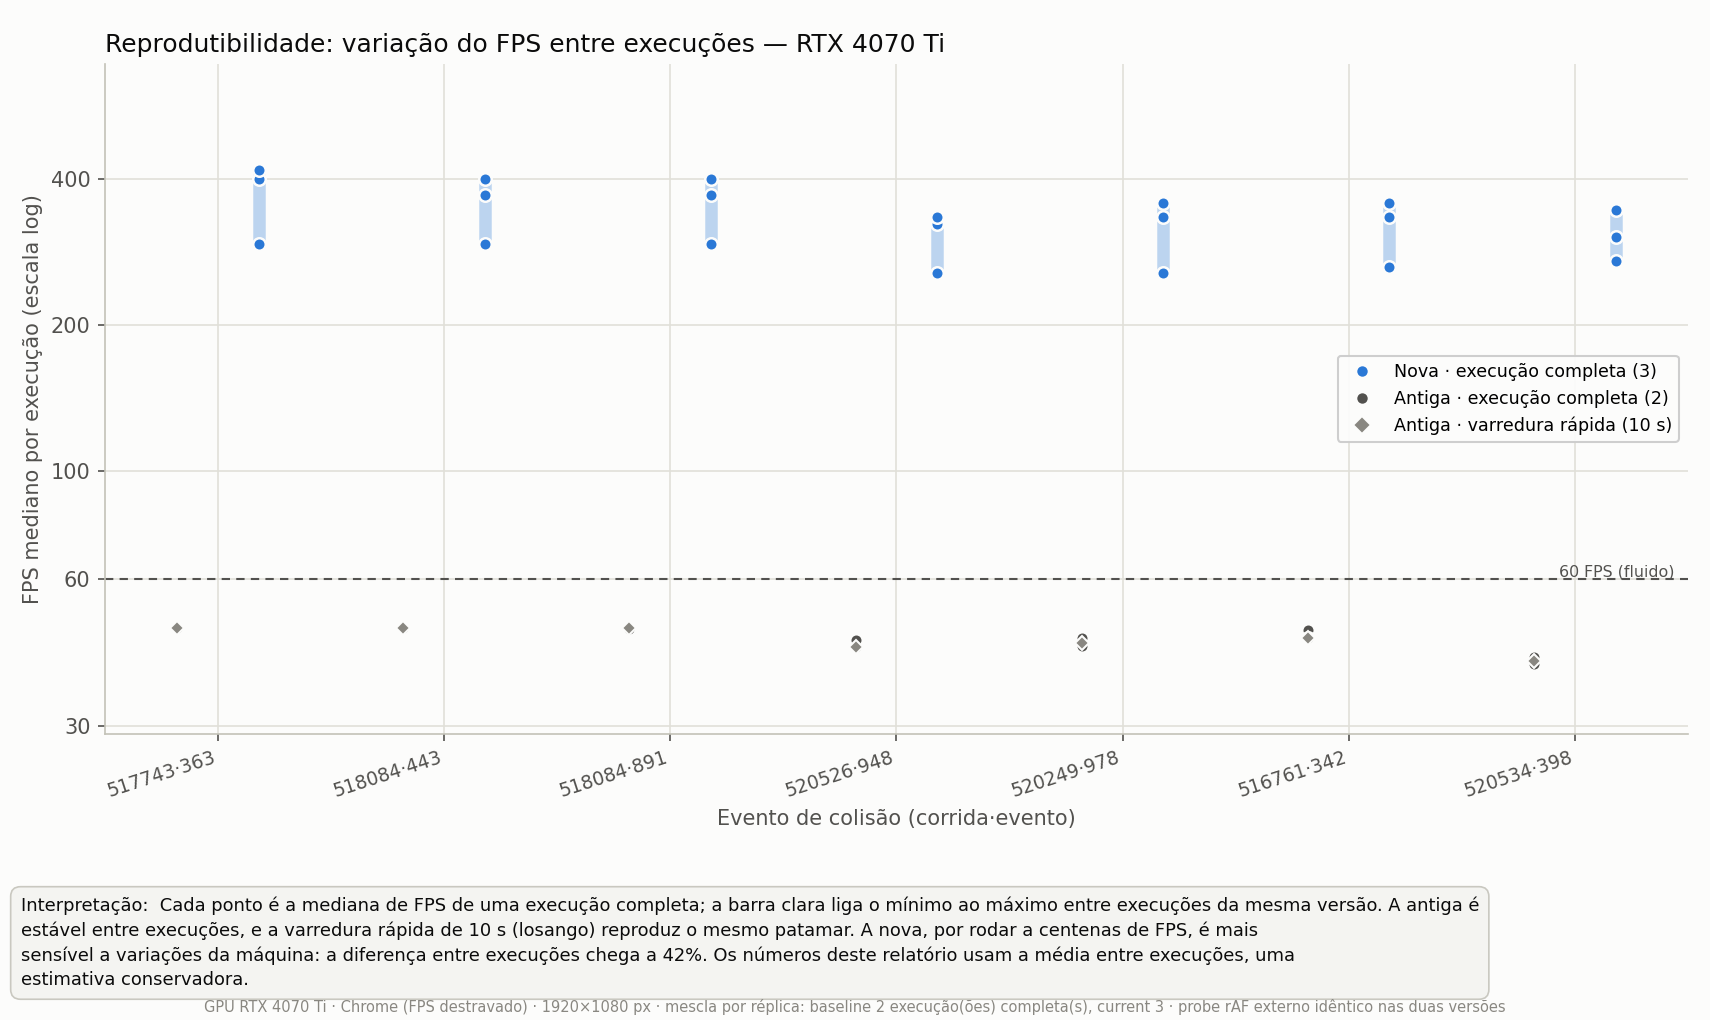
\includegraphics[width=0.9\linewidth]{12_reprodutibilidade.png}
  \caption{Variabilidade entre execu\c{c}\~oes: a antiga \'e est\'avel (e a varredura r\'apida
  de 10~s a confirma), enquanto o FPS da nova varia at\'e $42\%$ entre execu\c{c}\~oes,
  permanecendo sempre muito acima de 60~FPS.}
  \label{fig:repro-rtx}
\end{figure}

\begin{figure}[htbp]
  \centering
  
\includegraphics[width=0.85\linewidth]{08_drag.png}
  \caption{Arraste do plano de corte: de 8 a 10~FPS na vers\~ao antiga para 242~FPS na nova
  (m\'edia entre execu\c{c}\~oes). O eixo $\varphi$ s\'o existe na vers\~ao nova.}
  \label{fig:drag-rtx}
\end{figure}

\section{Conclus\~ao}

Na mesma m\'aquina e sob medi\c{c}\~ao externa id\^entica, mesclando cinco execu\c{c}\~oes
completas, as otimiza\c{c}\~oes (agrupamento de c\'elulas em lotes e corte na GPU) elevam o
CGV-Web de um regime consistentemente abaixo de 60~FPS, com intera\c{c}\~ao de corte a 8--10~FPS,
para centenas de FPS em todos os cen\'arios medidos: ganho t\'ipico de 10{,}4$\times$ e de at\'e
29$\times$ na intera\c{c}\~ao cr\'itica. A vers\~ao nova apresenta maior variabilidade entre
execu\c{c}\~oes (at\'e $42\%$), esperada em um aplicativo que passou a rodar a centenas de FPS,
mas at\'e o seu pior caso preserva uma folga larga sobre a vers\~ao antiga e sobre o limiar de
fluidez. Numa m\'aquina modesta (GTX~1050~Ti) o mesmo experimento rende
37$\times$ (relat\'orio pr\'oprio), confirmando que o ganho cresce quanto mais a CPU domina o
custo do quadro.

\end{document}
